\documentclass[11pt,a4paper]{article}
\usepackage[T1]{fontenc}
\usepackage[latin1]{inputenc}
\usepackage{a4wide}
\usepackage[dvips]{graphicx}

\usepackage[
pdfauthor={ACE Project Team},
pdftitle={Project Manual},
pdfcreator={pdftex},
]{hyperref}

\usepackage{sectsty}
\allsectionsfont{\sffamily}

\usepackage{fancyheadings} 
\pagestyle{fancy} 
\lhead{\textsf{\textbf{ACE} \\ \small{a collaborative editor}}}
\chead{}
\rhead{
\parbox[c]{3cm}{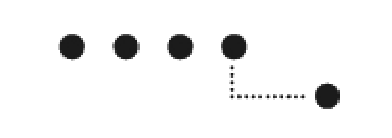
\includegraphics[height=0.875cm,width=3cm]{../../images/logo_BFH.eps}}
\parbox[c]{2.2cm}
{\tiny{\textsf{Berner Fachhochschule \\
Hochschule f�r \\
Technik und Informatik}}}}
\lfoot{}
\cfoot{\textsf{\thepage}}
\rfoot{}
\setlength{\headrulewidth}{0.6pt}
\setlength{\footrulewidth}{0.6pt}
\setlength{\topmargin}{-50pt}
\addtolength{\headheight}{50pt}

\usepackage{colortbl}

\newcommand{\headercol}[2]{\multicolumn{1}{|>{\bfseries\columncolor[gray]{0.82}}p{#1}|}{\textsf{#2}}}
\newcommand{\ace}[0]{\emph{ACE }}



\begin{document}

\begin{titlepage}
\thispagestyle{empty}
  
\includegraphics[height=1.5in]{../images/pix.eps}

  \begin{center}

    {\fontsize{40}{45} \textbf{\textsf{ACE}}} \\
    \textsf{a collaborative editor} \\
        
    \vspace{36pt}
        
    {\huge{\textbf{\textsf{}}}} \\

    \vspace{36pt}

	\textsf{Berne University of Applied Sciences} \\
    \textsf{School of Engineering and Information Technology} \\
    
  \end{center}

  \vfill
  
  \begin{tabular}{ll}
   \hline

   \\

   \multicolumn{1}{>{\bfseries}p{1.5in}}{\textsf{Date:}} &
   \multicolumn{1}{>{}p{4.3in}}{\textsf{08.11.2005}}          \\
   
   \\
   
   \multicolumn{1}{>{\bfseries}p{1.5in}}{\textsf{Version:}}     &   
   \multicolumn{1}{>{}p{4.3in}}{\textsf{0.1}}                 \\

   \\
   
   \multicolumn{1}{>{\bfseries}p{1.5in}}{\textsf{Projectteam:}}                 &
   \multicolumn{1}{>{}p{4.3in}}{\textsf{Mark Bigler (biglm2@hta-bi.bfh.ch)}}  \\
   \multicolumn{1}{>{\bfseries}p{1.5in}}{}                                      &
   \multicolumn{1}{>{}p{4.3in}}{\textsf{Simon Raess (rasss@hta-bi.bfh.ch)}}    \\
   \multicolumn{1}{>{\bfseries}p{1.5in}}{}                                      &
   \multicolumn{1}{>{}p{4.3in}}{\textsf{Lukas Zbinden (zbinl@hta-bi.bfh.ch)}} \\   
   
   \\
   
   \multicolumn{1}{>{\bfseries}p{1.5in}}{\textsf{Receivers:}}                       &
   \multicolumn{1}{>{}p{4.3in}}{\textsf{Jean-Paul Dubois (doj@hta-bi.bfh.ch)}}       \\
   \multicolumn{1}{>{\bfseries}p{1.5in}}{}                                          &
   \multicolumn{1}{>{}p{4.3in}}{\textsf{Claude Fuhrer (frc@hta-bi.bfh.ch)}}       \\

   \\
   
   \multicolumn{1}{>{\bfseries}p{1.5in}}{\textsf{Location:}}               &   
   \multicolumn{1}{>{}p{4.3in}}{\textsf{Subversion Repository}} \\

   \\  
   
   \hline
  \end{tabular}

\end{titlepage}


\section{Introduction}

\section{Project Documents}

\begin{itemize}
 \item System Requirements
 \item Project Manual (this document)
 \item User Manual
 \item Final Report
\end{itemize}

\subsection{System Requirements}
This document defines the goals and expected functionality of ACE - a collaborative editor.

\subsection{Project Manual}
The project manual contains:
\begin{itemize}
 \item list of delivered documents
 \item project plan: work phases, project organization
 \item used methods and tools
\end{itemize}

\subsection{User Manual}
The user manual contains:
\begin{itemize}
 \item instructions how to use the application
 \item instructions how to build and run the application
\end{itemize}

\subsection{Final Report}
The final report contains all the technical documentation of the project.
\begin{itemize}
 \item abstract
 \item description of goals and content of project
 \item description of implemented solution (implementation decisions)
 \item application architecture and design
 \item test concept and results
 \item references
 \item glossary
\end{itemize}

\section{Project Plan}

\subsection{Milestone Plan}

In the diploma project there are three milestones.

\subsubsection{Milestone M1}

The scheduled release date of Milestone 1 is: 21.11.2005. Milestone 1 includes the text editor with
all the discovery related functionality. Although it will be possible to publish local documents
it is not yet possible to join the shared documents.

\begin{itemize}
 \item create new documents
 \item load and save documents
 \item open multiple documents at the same time
 \item cut/copy/paste
 \item about information
 \item publish local documents
 \item automatic discovery of other running instances of ACE on a local area network (user discovery)
 \item automatic discovery of published documents of other running instances of ACE (document discovery)
\end{itemize}

\subsubsection{Milestone M2}

The scheduled release date of Milestone 2 is: 05.12.2005. Milestone 2 adds the collaboration functionality
to the text editor, including joining documents, collaborative editing, and awareness information.

\begin{itemize}
 \item join published documents
 \item collaborative editing in a shared document
 \item awareness information
 \item leave joined documents
 \item kick users
\end{itemize}

\subsubsection{Milestone M3}

The scheduled release date of Milestone 3 is: 12.12.2005. Milestone 3 incorporates mainly bugfixes and
usability improvements based on feedback from testing.

\begin{itemize}
 \item bug fixes
 \item usability improvements
 \item design
 \item optional goals
\end{itemize}


\section{Methods and Tools}

\subsection{Documentation}
To create the documentation, \LaTeX{} shall be used. Naturally, other applications are used for creating images and diagrams.
Because \LaTeX{} is a text-based format we can use SubEthaEdit (a collaborative editor for Mac OS X) and later even
ACE itself to collaboratively edit the documentation. 

\subsection{Source Repository}
Subversion is used as revision control system. The URL for Subversion access is
\href{http://ace.iserver.ch:81/repos/ace/ace}{http://ace.iserver.ch:81/repos/ace/ace}. The HEAD of the repository can
be browsed with a standard web browser.

\subsection{Website}
The project website's URL is \href{http://ace.iserver.ch}{http://ace.iserver.ch}. It is used mainly as a marketing instrument
for potential users. 

\subsection{Wiki}
We use the Confluence Wiki from http://www.atlassian.com/. It is available
at http://ace.iserver.ch:8080/confluence/. The Wiki is mainly used internally.

\subsection{Issue Tracker}
We use Jira from http://www.atlassian.com as issue tracker. It is available
at http://ace.iserver.ch:8080/jira/. The Issue Tracker is mainly used internally.

\subsection{Continous Integration}
We have a continous integration server (http://cruisecontrol.sourceforge.net/) that builds the
sources regularly and runs all the unit tests.

\subsection{Development}
\begin{itemize}
 \item Eclipse (http://www.eclipse.org/)
 \item SubEthaEdit (http://www.codingmonkeys.de/subethaedit/)
 \item ant (http://ant.apache.org/)
 \item CruiseControl (http://cruisecontrol.sourceforge.net/)
\end{itemize}


\section{Standards and Guidelines}

\subsection{Documentation}
All \LaTeX{} documents must include the file \texttt{ace.tex}. This file can be found in the subversion repository at \texttt{/ace/trunk/doc/latex/ace.tex}.
A template for all \LaTeX{} documents is in the same directory (\texttt{template.tex}). There is also a template for titlepages (\texttt{template.tex}).

\subsection{Source Code}
The documentation of the source code is done with JavaDoc. The comments must be written in English. Source code files must have the following standard header,
which can be found at \texttt{/ace/trunk/doc/templates/source.header} in the Subversion repository.

\small{
\begin{verbatim}
/*
 * $Id$
 *
 * ace - a collaborative editor
 * Copyright (C) 2005 Mark Bigler, Simon Raess, Lukas Zbinden
 *
 * This program is free software; you can redistribute it and/or
 * modify it under the terms of the GNU General Public License
 * as published by the Free Software Foundation; either version 2
 * of the License, or (at your option) any later version.
 *
 * This program is distributed in the hope that it will be useful,
 * but WITHOUT ANY WARRANTY; without even the implied warranty of
 * MERCHANTABILITY or FITNESS FOR A PARTICULAR PURPOSE.  See the
 * GNU General Public License for more details.
 *
 * You should have received a copy of the GNU General Public License
 * along with this program; if not, write to the Free Software
 * Foundation, Inc., 59 Temple Place - Suite 330, Boston, MA  02111-1307, USA.
 */
\end{verbatim}
}

\subsubsection*{Conventions}

The source code files shall be edited according to the Sun Coding Conventions (\href{http://java.sun.com/docs/codeconv/}{http://java.sun.com/docs/codeconv/}).
The indendation uses tab characters (not spaces!).

\end{document}


\end{document}
